  The real results
 % \missingfigure{This is a place holder figure}
  This figure is to show that for one sample of one shot pruning we can
  outperform deterministic pruning for pruning rate 0.8
\begin{figure}[tb]
    \centering
    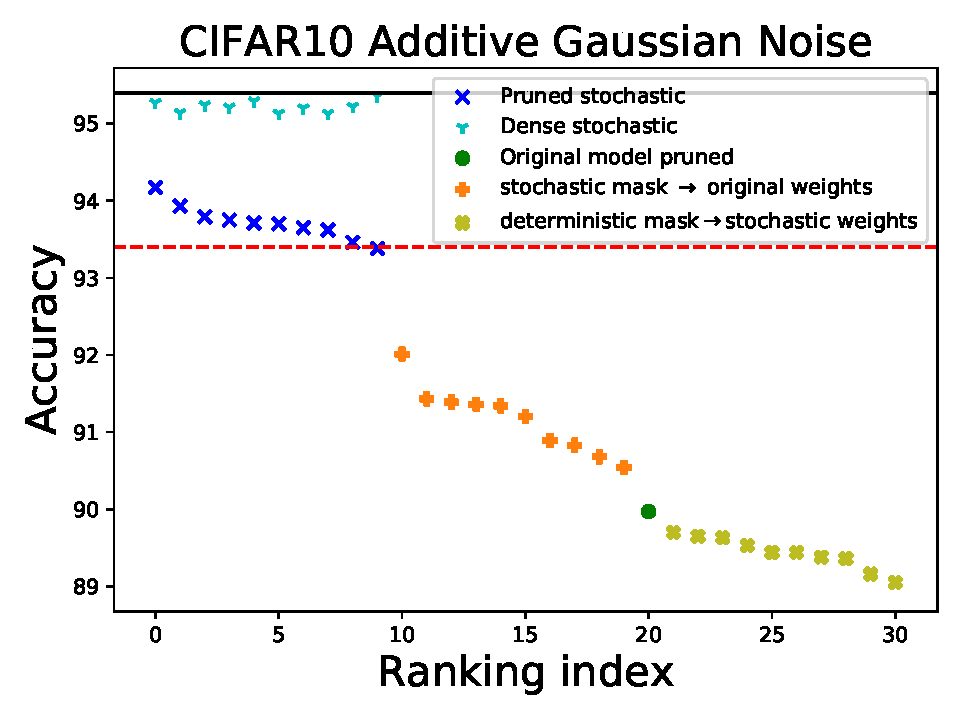
\includegraphics[width=0.8\textwidth]
    {transfers_comparison_gaussian_sigma_0.0021419609859022197_pr_0.8_batchSize_512_pop_10_t_14-29.pdf}
    \caption{}
    \label{fig:}
\end{figure}


The next 3 figures are to show that this is not a "lucky" sample. That this
phenomena is persistent across pruning rates and across noise levels.
\begin{figure}[tb]
    \centering
    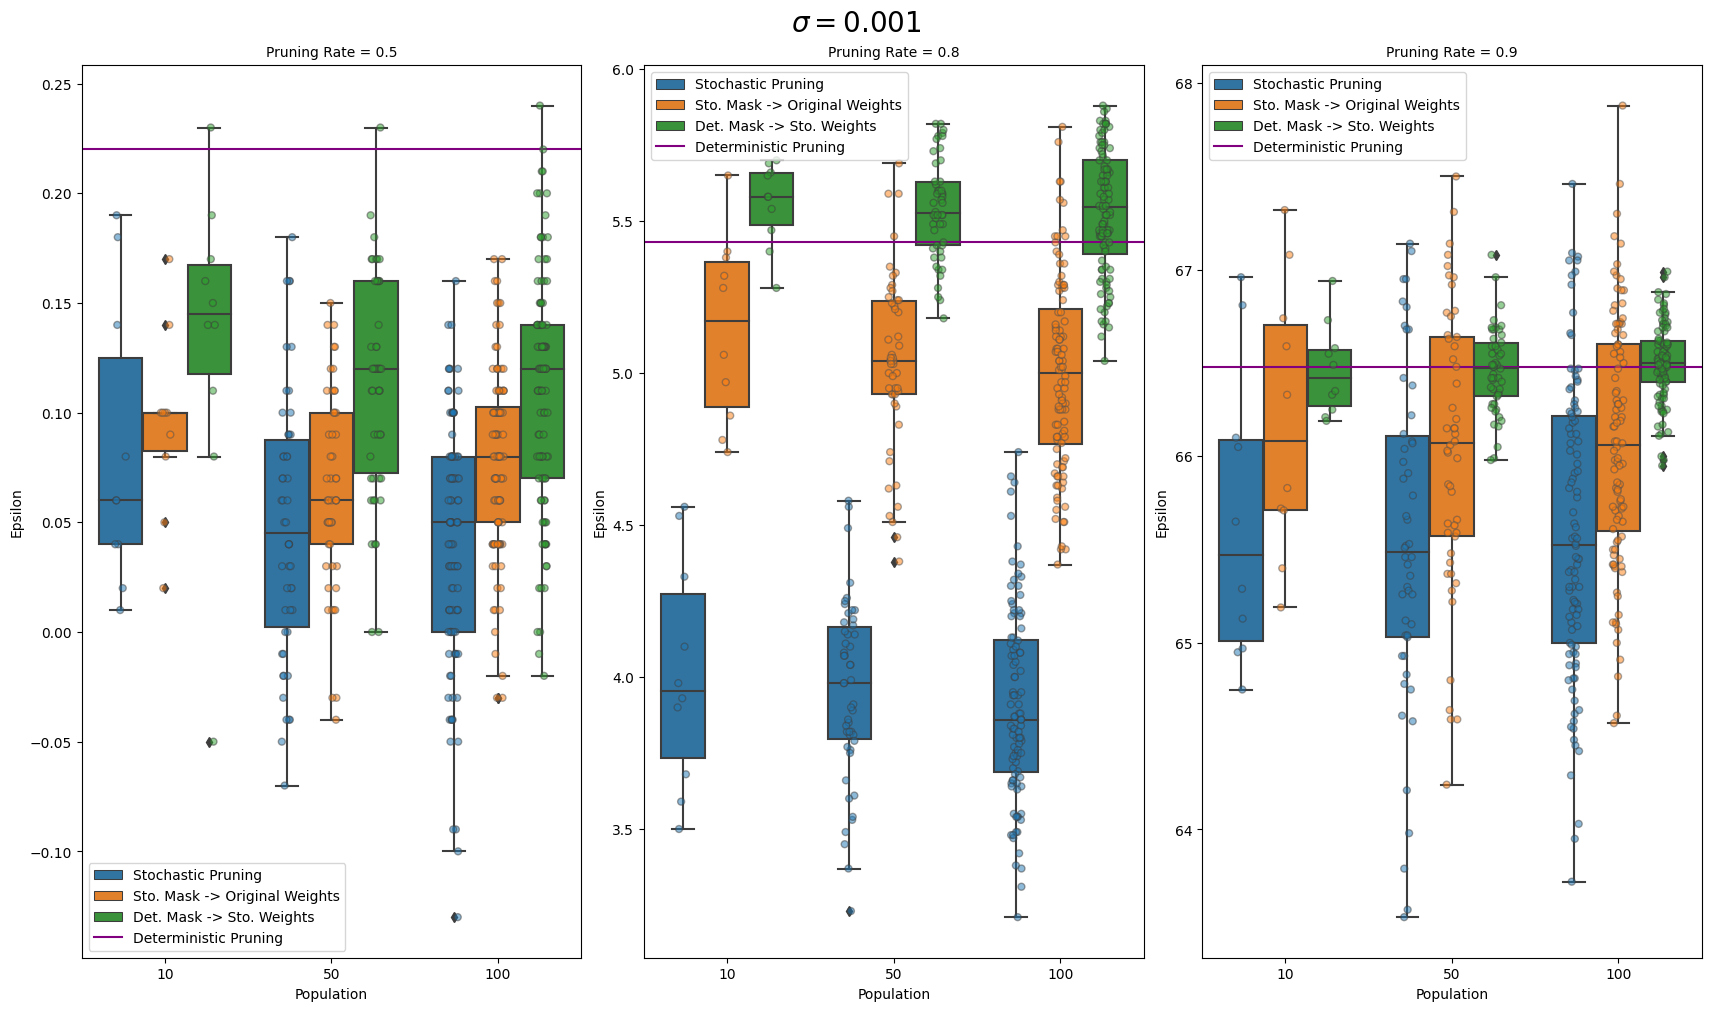
\includegraphics[width=0.8\textwidth]{epsilon_allN_all_pr_sigma=0.001.png}
    \caption{Accuracy degradation for one-shot stochastic pruning $\sigma=0.001$}
    \label{fig:OS0.001}
\end{figure}
\begin{figure}[tb]
    \centering
    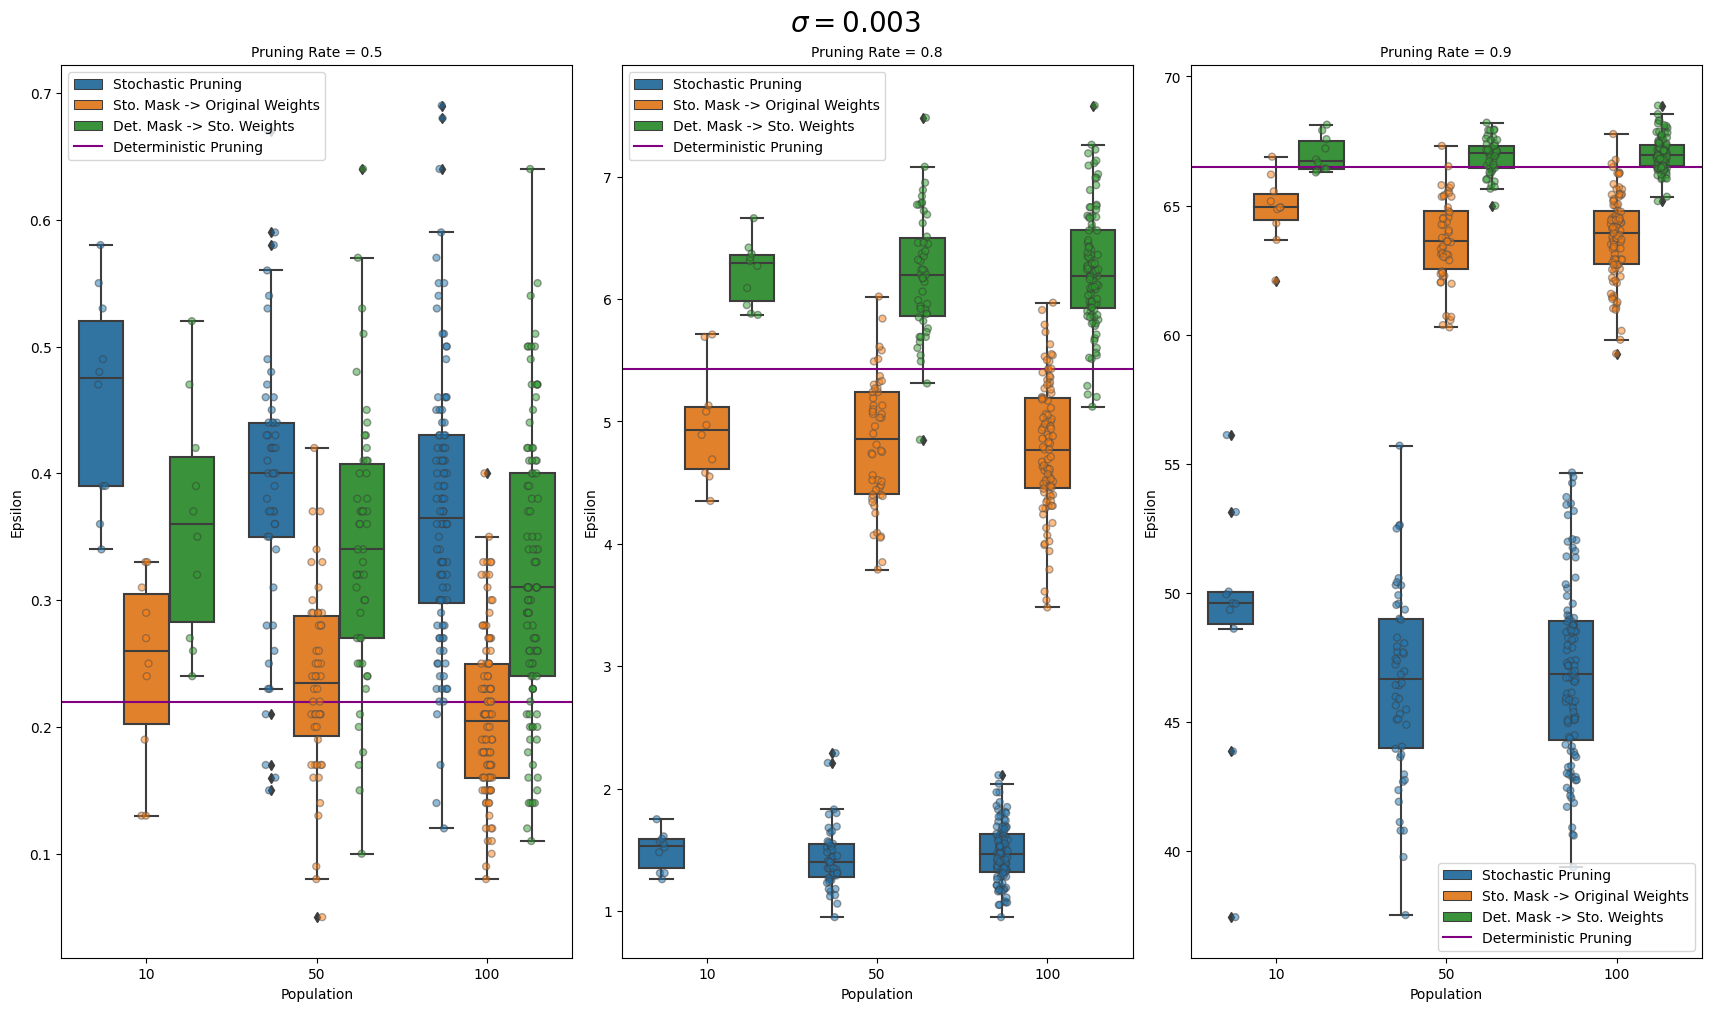
\includegraphics[width=0.8\textwidth]{epsilon_allN_all_pr_sigma=0.003.png}
    \caption{Accuracy degradation for one-shot stochastic pruning $\sigma=0.003$}
    \label{fig:OS0.003}
\end{figure}

\begin{figure}[tb]
    \centering
    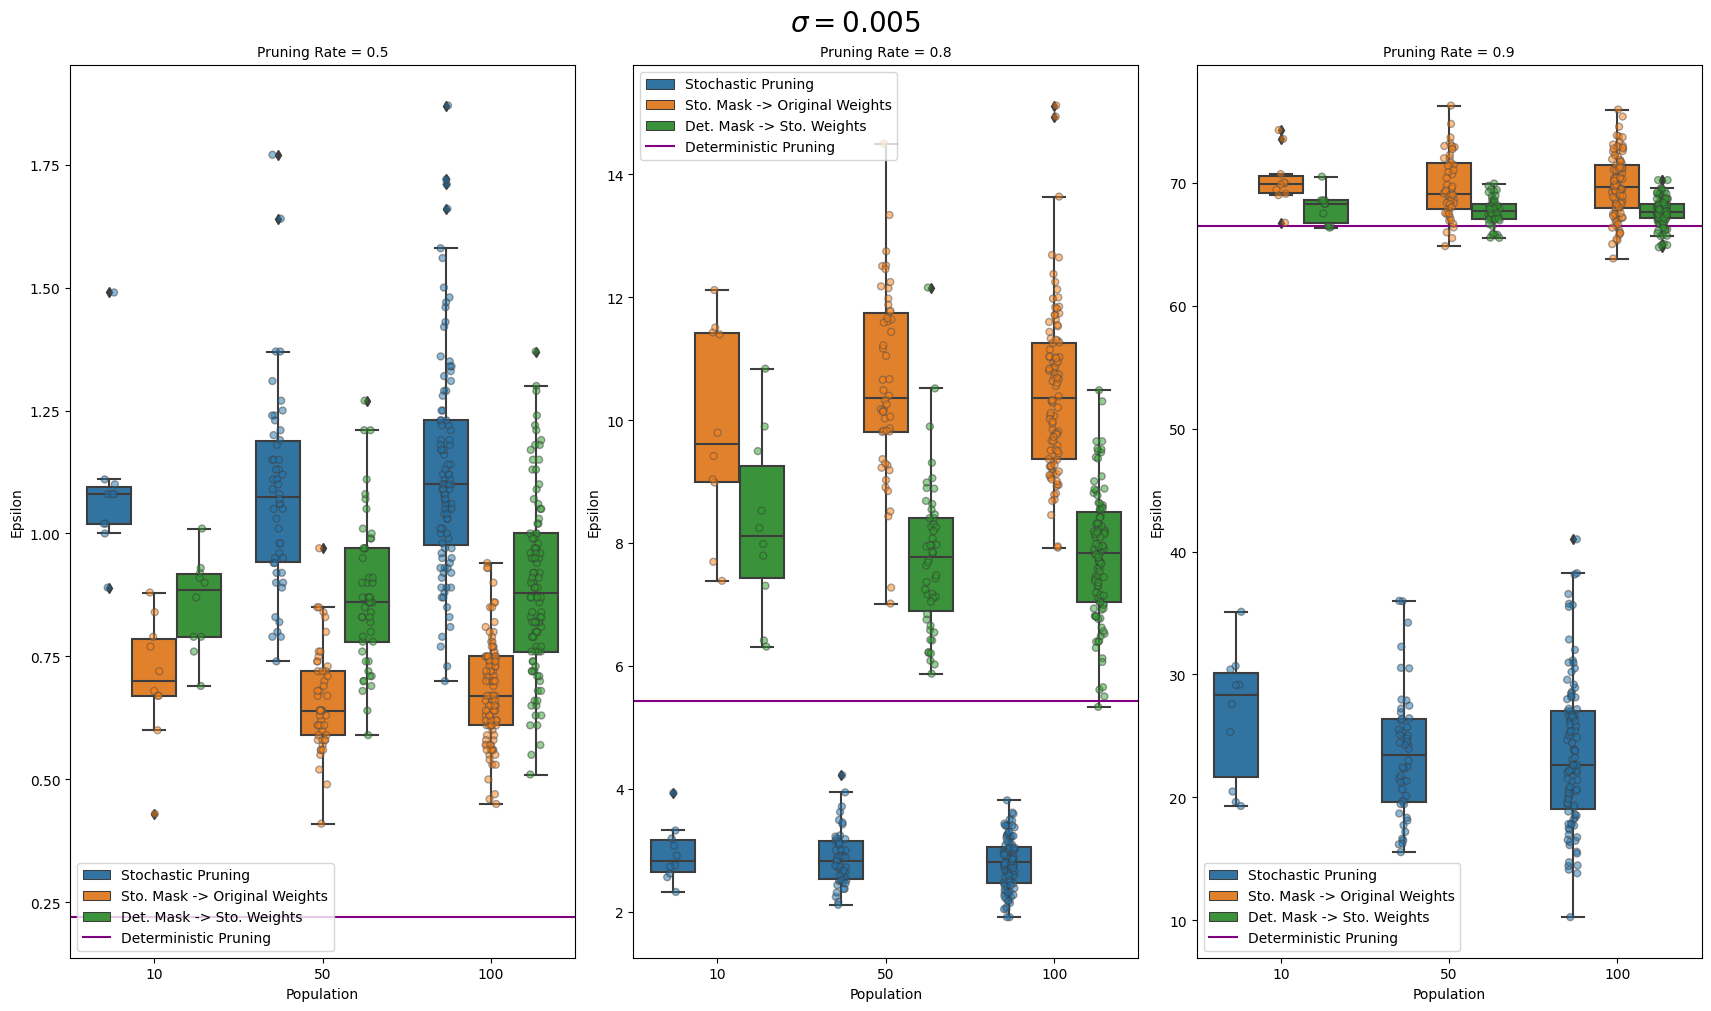
\includegraphics[width=0.8\textwidth]{epsilon_allN_all_pr_sigma=0.005.png}
    \caption{Accuracy degradation for one-shot stochastic pruning $\sigma=0.005$}
    \label{fig:OS0.005}
\end{figure}
  %\begin{figure}[ht]
  %    \centering
  %    \includegraphics[width=\columnwidth]
  %    {epsilon_allN_all_pr_sigma=0.001.png}
  %    \caption{Epsilon for $\sigma=0.001$ varying population size and different
  %    pruning rates}
  %    \label{fig:allNS0.001}
  %\end{figure}
  %\begin{figure}[ht]
  %    \centering
  %    \includegraphics[width=\columnwidth]
  %    {epsilon_allN_all_pr_sigma=0.003.png}
  %    \caption{Epsilon for $\sigma=0.003$ varying population size and different
  %    pruning rates}
  %    \label{fig:allNS0.003}
  %\end{figure}
  %\begin{figure}[ht]
  %    \centering
  %    \includegraphics[width=\columnwidth]
  %    {epsilon_allN_all_pr_sigma=0.005.png}
  %    \caption{Epsilon for $\sigma=0.005$ varying population size and different
  %    pruning rates}
  %    \label{fig:allNS0.005}
  %\end{figure}
